% generation d'un .a que tu peux utiliser en ajoutant USE_STATIC_LIB=1 dans ton Makefile
% ajouter LDFLAGS+=-liio dans Makefile cree par module_generator

% device_reboot sf
% dfu-util -a firmware.dfu -D pluto.dfu

% dans le .dts : on remplace target = <&fpga_full>; par target = <&fpga_axi>; et on commente le nom du bitstream

\documentclass[12pt,oneside]{article}
\usepackage{makeidx,anysize,mflogo,xspace,float,epsfig,url}
\usepackage{amsmath,amsfonts,amssymb,a4wide} 
\usepackage[utf8]{inputenc}
%\usepackage[francais]{babel}
%\usepackage[french]{babel}
\urlstyle{sf}
%\usepackage{subcaption}
\usepackage{hyperref}
\usepackage{graphicx}
\usepackage{graphics}
\usepackage{float}
\usepackage{caption}
\usepackage{colordvi} %??
\usepackage{listings} 
\usepackage{subfigure}
\usepackage{subfloat}
\usepackage{xcolor}
\graphicspath{{./figures/}}
%\usepackage[labelsep=quad,indention=10pt]{subfig}
\definecolor{grey}{rgb}{0.95,0.95,0.95} % on définit la couleur grise
	% (c'est un gris très clair)
	\definecolor{red}{rgb}{1.0,0.0,0.0} 
	\definecolor{green}{rgb}{0.0,1.0,0.0}
	\definecolor{blue}{rgb}{0.0,0.0,1.0}
	\lstloadlanguages{bash,Java,C,C++,csh,make,sh}%%[Visual]Basic,xml}
	\lstset{frame=none,basicstyle=\footnotesize,breaklines,tabsize=2,captionpos=b,
		prebreak={\hbox{$\rightarrow$}},postbreak={\hbox{$\hookrightarrow$}},
		showstringspaces=false,backgroundcolor=\color{grey}\bfseries,
		keywordstyle=\color{blue},commentstyle=\color{green}\textit,
		stringstyle=\color{red}\ttfamily,abovecaptionskip=2pt,aboveskip=0pt,
		belowskip=0pt,belowcaptionskip=0pt,numbers=none,columns=fullflexible, backgroundcolor=\color{grey}}
%left,numberstyle=\footnotesize,
%		stepnumber=2,numbersep=1pt}

\begin{document}


\begin{center}
{\bf \Large Using ADALM-PLUTO within \\ the OscimpDigital Ecosystem} \\ \ \\
P.-Y. Bourgeois \\ \href{mailto:pyb2@femto-st.fr}{pyb2\_at\_femto-st.fr}\ \\ \today
\end{center}


This tutorial is intended to help you to handle the ADALM-PLUTO board within the
OSCIMP framework.
It is focused on

\begin{itemize}
	\item Providing general guidelines to set up the environment
	\item Performing a Pluto's harware independant check (NCO$\to$RAM, check the data)
	\item Connecting the Pluto data stream into the RAM and recovering the data
\end{itemize}

\begin{figure}[h!]
	\centering{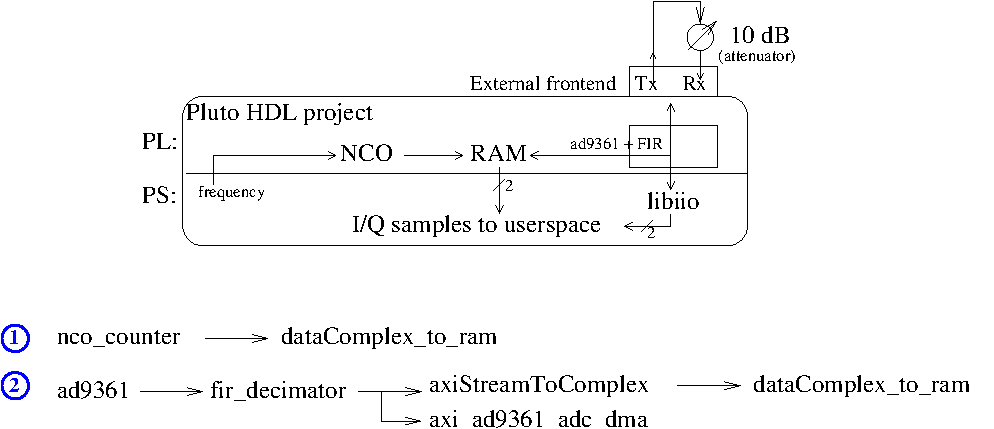
\includegraphics[width=\linewidth]{pluto-oscimpDigital-objective}
		\caption{Objectives of this tutorial and raw schematics of the
processing chains.}}
\end{figure}


%-----------------------------------
\section*{Disclaimer}
%-----------------------------------
Neither the author nor the developpers of the OSCIMP repositories shall be
responsible for misuse of the presented Software and Hardware.
All the given codes and guidelines of this tutorial are provided 'as is'.



%-----------------------------------
\section{Objectives / Experimental set-up}
%-----------------------------------

Right out of the box, the ADALM-PLUTO board, when fired up, is able to be fully
configurable and flawlessly accessible thanks to \emph{iio} contexts of the {\bf{libiio}}.
Thanksfully AnalogDevicesInc provide the library but also distribute the HDL
code:)
It becomes then interresting to test the compatibility of the original Pluto HDL
project within the OSCIMP ecosystem and beneficiate for extra HDR/SDR features.

For this tutorial, we want to recover I/Q samples of a 100 kHz beatnote. Achieving this
result is first assessed by fetching samples from the output of a 100~kHz NCO operating
independently of the AXI Stream provided by ADI. Having checked that the samples are
properly generated and recovered, we mix the output of the AXI Stream including the
I/Q coefficients from the AD9363 and check that the result is consistent. Thus:

\begin{itemize}
\item the first part aims at checking the correct bitstream synthesis of the project
provided by ADI using an additional NCO and RAM transfer from the OSCIMP
ecosystem. In this setup (called sanity check), the NCO acts as a fake 100~kHz
beatnote generator, the added IPs having no relationship with the initial
firmware,
\item in the second part, we connect custom blocks to the AXI Stream from the
AD9363 and demonstrate how custom processing can be added to the original ADI processing chain.
\end{itemize}


In order to create a ``beatnote'', one can use the following setup:

%\begin{figure}[h!]
\begin{minipage}[c]{0.49\linewidth}
	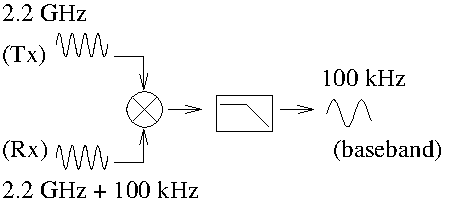
\includegraphics[width=\linewidth]{beatnote_pluto_scheme.pdf}
\end{minipage}\hfill
\begin{minipage}[c]{0.49\linewidth}
	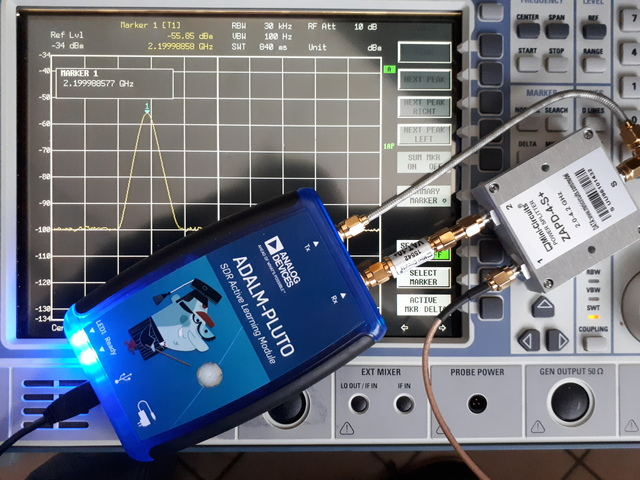
\includegraphics[width=\linewidth]{20190213_105039_640.jpg}
\end{minipage}
%\end{figure}

The {\bf Tx} port of the PlutoSDR board is set to transmit at 2.2 GHz. When connecting
the PlutoSDR Sink (select an input level lower than 1 to avoid saturation and 
unwanted signal beyond the carrier), the Tx transmits nothing but the carrier at 2.2 GHz 
(i.e. with no signal of interrest nor message). The receiver part is slightly detuned at 
$2.2$~GHz$+100$~kHz. After demodulation (RF-hardware) and decimating filter ({\tt fir\_decimator}
block within the PL-side of the FPGA), a remaining ``beatnote'' at $f_b=100$~kHz occurs.
Once we know in advance the frequency of this beatnote, when the sampling rate
is set up at $fs=50$~MHz ({\bf JUSTIFIER : AXI Stream clock bus}), we also know that a window 
of $N=2048$ samples will present around 4 periods of the beatnote ($N/fs/fb$).
This ``beatnote'' trick is  an easy trick that is routinely used when developping
RF applications, to check the correctness of the data.

On the photography, a splitter has been added (before the 10~dB attenuator) to also send the 
{\bf Tx} port on a spectrum analyzer which enable to check if the right transmit carrier frequency 
has been set up through {\it iio}. 
% comprends pas le sens ci-dessous, comme on ne voit pas l'echelle de la courbe l'ecart entre
% TX LO et RX LO n'est pas visible ... ne me semble pas utile
%Obviously the peak measure does not show a $\sim$round 2.20 GHz
%frequency because the pluto and the spectrum analyzer embed different clocking
%systems that are further not referenced to an atomic reference.

%-----------------------------------
\section{Setting up the environment}
%-----------------------------------
To complete this tutorial, we suppose some experience in using the \mbox{OSCIMP} ecosystem has
been acquired. Also up to date versions of the following repositories must be fetched:
	\begin{itemize}
		\item oscimpDigital (\href{https://github.com/oscimp/oscimpDigital}{https://github.com/oscimp/oscimpDigital}). Remember to recursively clone the repository\\
{\tt git clone --recursive https://github.com/oscimp/oscimpDigital} \\
and set the {\tt BOARD\_NAME} to redpitaya since the PlutoSDR is fitted with the same Zynq model than
the Redpitaya
		\item The BR2\_EXTERNAL framework for Analog Device's PlutoSDR Zynq \\ (\href{https://github.com/oscimp/PlutoSDR}{https://github.com/oscimp/PlutoSDR})
		\item The HDL project from analogDevices (see further below).
	\end{itemize}

In order to build the HDL project for the ADALM-PLUTO board, only the {\bf{hdl}} repository
(\href{https://github.com/analogdevicesinc/hdl}{https://github.com/analogdevicesinc/hdl}) is needed.
% but it is recommended to checkout the conservative commit used in
% \href{https://github.com/analogdevicesinc/plutosdr-fw}{https://github.com/analogdevicesinc/plutosdr-fw}. 
% JMF : je vire car inutile (cf hash ci-dessous en cas de doute)

\smallskip
At the time of writing (\today), the following versions are functional:
	\begin{itemize}
		\item {\bf{adi\_hdl}} branch {\bf{hdl\_2018\_r2}} (401395cdd1980827fd1f7043ce1a10770f666c64)
		\item Vivado 2018.3
	\end{itemize}


To build the HDL project for the Pluto board, {\tt source} the
{\tt settings64.sh} script of your Vivado 2018.2, and {\tt make} the
{\tt /somewhere\_analogdevicesinc/hdl/projects/pluto}.

(On some computers, several {\tt make} in a row are required to undergo some error messages). 

A successful build of the HDL project is returned by the console message:\\
\noindent {\tt
Building {\bf{pluto}} project
[/pathTo\_adi\_hdl/projects/pluto/pluto\_vivado.log] ... {\bf{OK}}
}


%-----------------------------------
\section{Sanity check (NCO$\to$RAM$\to$UserSpace)}
%-----------------------------------
This tutorial allows us to use the OscimpDigital blocks with the embedded Zynq of
the PlutoSDR board. It is seen as a first-step demonstration of compatibility.

\subsection{Design}

Once the pluto HDL project is successfully built, open \emph{pluto.xpr} within
Vivado. 

Add the \emph{oscimpDigital/fpga\_ip} repository (Icon ``Settings'' $\to$ ``Project
Settings'' $\to$ ``IP'' $\to$ ``Repository'' $\to$ + then Apply and close the window).

Open the block design, right-click, ``Add IP'', then add the \emph{dataComplex\_to\_ram} 
and \emph{nco\_counter}. Run the ``Connection Automation'': the NCO counter and dataComplex\_to\_ram
should connect to the AXI bus and have addresses assigned to their registers: dataComplex\_to\_ram
base address should be 0x43C0\_0000 and nco\_counter base address should be 0x43C1\_0000. 
If adresses mismatch, keep them in mind as you will need it for the Device Tree overlay.

The next step is to configure the added IPs: %as shown in Fig. \ref{configs}, 
we set
\begin{itemize}
\item the NCO block {\tt Data Size} to 16~bits, {\tt Counter Size} to 28~bits, and {\tt LUT
Size} to 10~bit,
\item the Data Complex to RAM block with {\tt Data Size} to 16~bits, {\tt Number of Inputs}
to 1, and {\tt Number of Samples} to 1024. % JMF/GGM : j'ai 1024 et non 2048 echantillons/voie
\end{itemize}

%\begin{figure}[h!]
%\begin{minipage}[c]{0.49\linewidth}
%	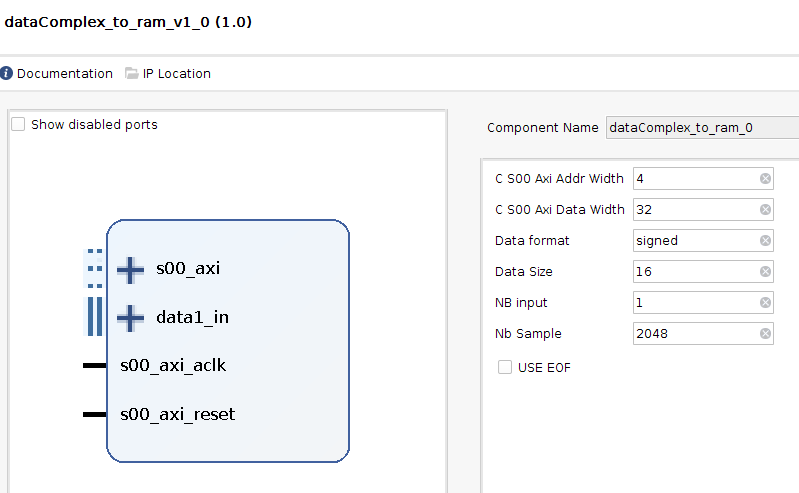
\includegraphics[width=\linewidth]{2019-02-12-165739_799x493_scrot.png}
%\end{minipage}\hfill
%\begin{minipage}[c]{0.49\linewidth}
%	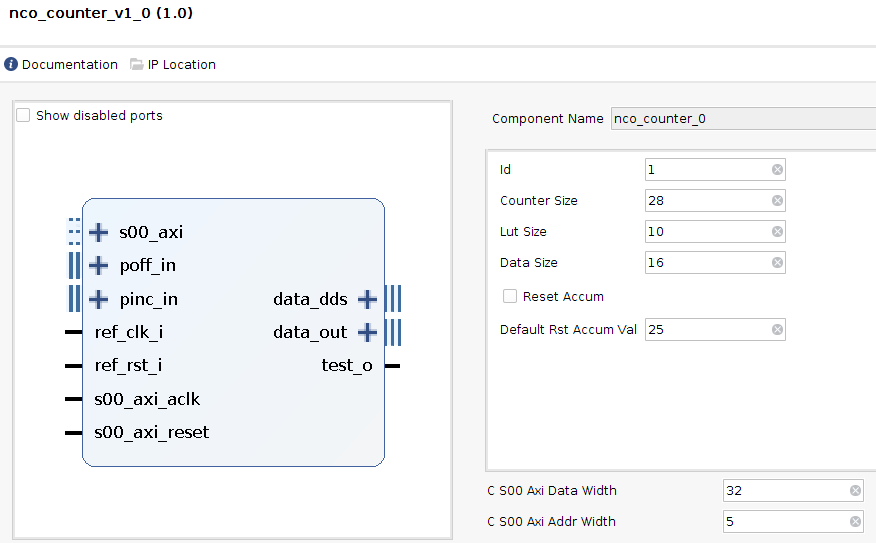
\includegraphics[width=\linewidth]{2019-02-12-170033_876x543_scrot.png}
%\end{minipage}
%\label{configs}
%\end{figure}

Additional connections (Fig. \ref{con}):

\begin{itemize}
\item NCO
	\begin{itemize}
	\item {\tt ref\_rst\_i} $\to$ {\tt s00\_axi\_reset} on the same block
	\item {\tt ref\_clk\_i} $\to$ {\tt s00\_axi\_aclk} which refers to the PS7's
FCLK\_CLK0 at 100~MHz. We might as well clock and reset all blocks on the AD936x signals.
	\end{itemize}
\item NCO $\to$ RAM
        \begin{itemize}
	\item {\tt sine\_out} $\to$ {\tt data1\_in} % JMF : changement de nom de la sortie
        \end{itemize}
\end{itemize}

\begin{figure}[h!tb]
%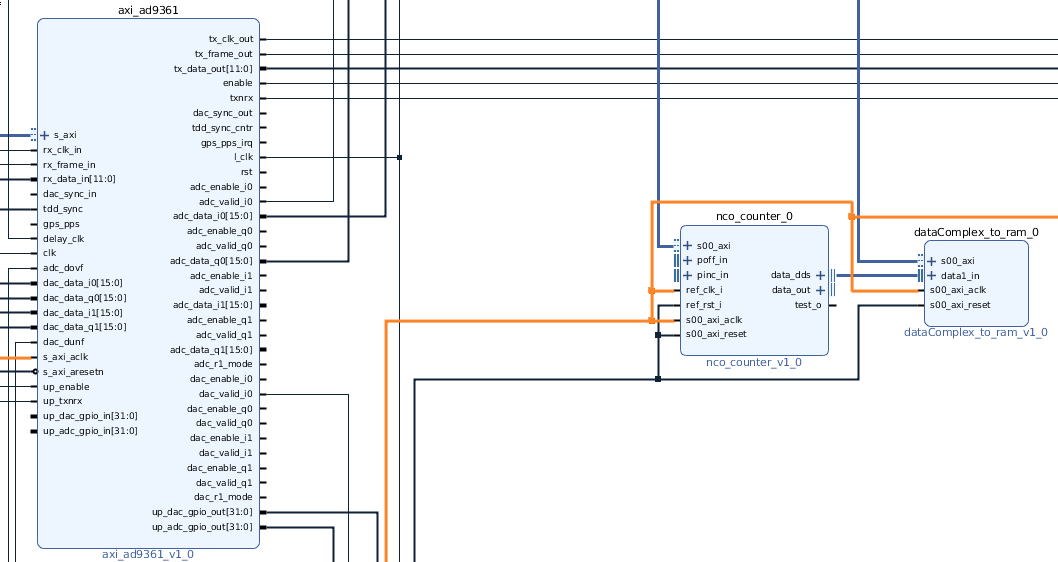
\includegraphics[width=.7\linewidth]{2019-03-07-091613_1058x562_scrot.png}%2019-02-12-171957_1072x583_scrot.png}
\begin{center}
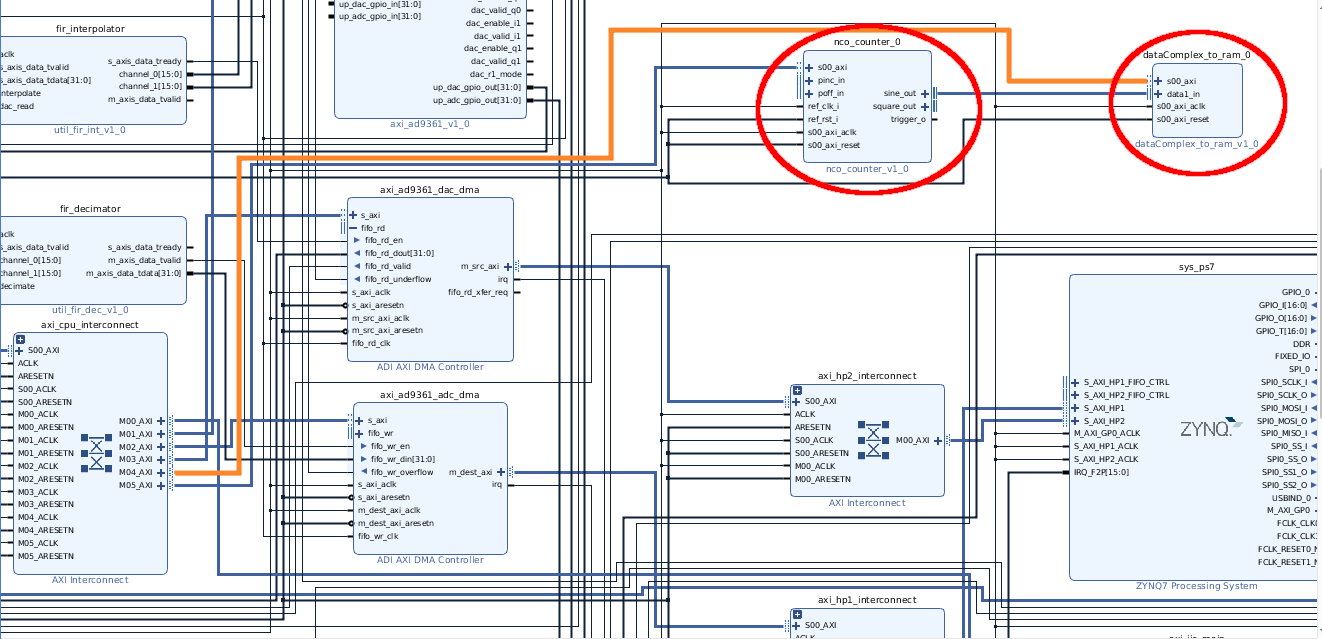
\includegraphics[width=\linewidth]{1.png}
\end{center}
\caption{Connection of the custom blocks to the PlutoSDR firmware.}
\label{con}
\end{figure}

At last, click on ``Generate Bitstream'', and once the synthesis is done, place
the {\tt /pathTo\_adi/hdl/projects/pluto/pluto.runs/impl\_1/system\_top.bit}
into the \\{\tt /somewhere/PlutoSDR/board/pluto} BR2\_EXTERNAL directory.

%--------------------------------
\subsection{Oscimp library / Linux Drivers}
%--------------------------------
The library {\bf{liboscimp\_fpga}} should be compiled for your environment. We have selected
to statically link the library to the application to avoid confusion with multiple library
versions: when compiling the userspace application using the {\tt Makefile} provided by
{\tt module\_generator} (see below) by adding {\tt USE\_STATIC\_LIB=1} after the
{\tt BASE\_NAME}

Also both drivers for the NCO ({\tt nco\_counter\_core.ko}) and RAM ({\tt
data\_to\_ram\_core.ko}) should be compiled. 

%--------------------------------
\subsection{Device Tree Overlay}
%--------------------------------

%The linux-side of the Pluto board uses the Device Tree overlays mechanism to
%affect the kernel side tree which allows for PL configuration dynamically.
%
%All we have to do is to indicate the presence of the NCO and RAM into the Device
%Tree structure. 
%A dirty but efficient way to do this is to edit the {\bf{zynq-pluto-sdr.dtsi}}
%that stands in \emph{/pathTo/buildroot-2018.11.1/output/build/linux-something/arch/arm/boot/dts/}
%
%%../../zynq-pluto-sdr.dtsi -> buildroot-2018.11.1/output/build/linux-c2041af164e263d852897cf90edb5cca9f677579/arch/arm/boot/dts/zynq-pluto-sdr.dtsi
%
%
%and eventually change the addresses accordingly:
%\begin{verbatim}
%
%/ {
%        fpga_axi: fpga-axi@0 {
%                compatible = "simple-bus";
%                #address-cells = <0x1>;
%                #size-cells = <0x1>;
%                ranges;
%
%                axi_i2c0: i2c@41600000 {
%
%...
%...
%
%                data2ram: data2ram@43c00000{
%                        compatible = "ggm,dataToRam";
%                        reg = <0x43c00000 0xffff>;
%                };
%
%                nco00: nco00@43c10000{
%                        compatible = "ggm,nco_counter";
%                        reg = <0x43c10000 0xffff>;
%                };
%
%        };
%};
%
%&spi0 {
%        status = "okay";
%...
%...
%\end{verbatim}

The devicetree overlay will be generated by {\tt modules\_generator}: the configuration
file ({\tt config.xml}) looks like
{\footnotesize
\begin{verbatim}
<?xml version="1.0" encoding="utf-8"?>
<drivers name="PlutoSDR_custom" version="1.0">
  <driver name ="data_to_ram" >
    <board_driver name="data00" id = "0" base_addr="0x43c10000" addr_size="0xffff" />
  </driver>
  <driver name ="nco_counter" >
     <board_driver name="nco00" id = "0" base_addr="0x43c00000" addr_size="0xffff" />
  </driver>
</drivers>
\end{verbatim}
}
where {\tt data00} and {\tt nco00} are the {\tt /dev} entries and the base addresses
should match thoses provided by Vivado. A few updates must be brought to the output
of {\tt module\_generator} after running {\tt module\_generator -dts config.xml}
\begin{itemize}
\item in dans le {\tt .dts}: replace \verb~target = <&fpga_full>;~ with \verb~target = <&fpga_axi>;~ 
and comment out the bitstream name
\item in the {\tt Makefile}, add {\tt USE\_STATIC\_LIB=1} and {\tt LDFLAGS+=-liio} after the project
name but prior to the {\tt Makefile.inc} inclusion
\item in the shell script, comment the lines creating the firmware directory and attempting to copy
the bitstream to this location.
\end{itemize}

The last step is then to rebuild the firmware ({\tt pluto.frm}) :

\begin{itemize}
	\item remember that we have copied the bitstream to the PlutoSDR
directory in \\
{\tt /somewhere/PlutoSDR/board/pluto}, hence providing buildroot with the appropriate
bitstream named {\tt system\_top.bit}.
	\item {\tt cd pathTo/buildroot-version/}
%	\item {\tt touch output/build/linux-something/.config} % JMF ne me semble pas utile
	\item {\tt make}
\end{itemize}

%--------------------------------
\subsection{Flash the pluto}
%--------------------------------

\paragraph{NB:} For the moment, the repository PlutoSDR provides only support
for rootfs and linux (the bootloader part still remains to be added). Hence, any
change of the bistream requires to perform the steps presented here:

\begin{itemize}
	\item Fire up the PlutoSDR // wait for the mass-storage to be available (via
{\tt dmseg -w} for example)
	\item {\tt mount /dev/sdX1\footnote{X is the index of the pluto mass-storage, e.g.
/dev/sde1} /mnt/somewhere/}
	\item {\tt cp pathTo/buildroot-version/output/images/pluto.frm /mnt/somewhere/}
	\item {\tt eject /dev/sdX1}  % JMF : moi j'ai toujours fait sdX : est-ce correct ?
\end{itemize}

You should see the {\bf \textcolor{blue}{blue LED1}} flashing quickly, thus do not disconnect
nor touch anything until the PlutoSDR has rebooted or you may brick the board at
this stage. 

Alternatively, the DFU image can be transfered to the PlutoSDR flash by rebooting,
from the target GNU/Linux prompt, to DFU mode with
{\footnotesize
\begin{verbatim}
device_reboot sf
\end{verbatim}
}
and then running on the host personnal computer
{\footnotesize
\begin{verbatim}
dfu-util -a firmware.dfu -D my_pluto_firmware.dfu
\end{verbatim}
}
with {\tt my\_pluto\_firmware.dfu} matching the name of the image to be flashed. Again wait for
the transfer to complete and the message stating that no error was detected to appear.

The PlutoSDR is now ready to be tested.

%--------------------------------
\subsection{Application}
%--------------------------------

The application-side makes use of \emph{libiio} as well as \emph{liboscimp}. For
the former, one can find examples from M. Hennerich presentation at GNU Radio
Conference 2018

\href{https://www.gnuradio.org/grcon/grcon18/presentations/plutosdr/}{https://www.gnuradio.org/grcon/grcon18/presentations/plutosdr/}

or following guidelines written in the ADI wiki website

\href{https://wiki.analog.com/resources/tools-software/linux-drivers/iio-transceiver/ad9361}{https://wiki.analog.com/resources/tools-software/linux-drivers/iio-transceiver/ad9361}

and 

\href{https://wiki.analog.com/university/tools/pluto/controlling\_the\_transceiver\_and\_transferring\_data}{https://wiki.analog.com/university/tools/pluto/controlling\_the\_transceiver\_and\_transferring\_data}

to tweek the configuration.

For this part, we have just changed Hennerich's snippet code to the desired
configuration of TX and RX carriers, Sampling rate, the ``process'' part only
consists of writing the ram buffer into a data file.

An example file is provided in the folder {\bf{get\_data/nco\_data2ram}}. Running this example
requires loading the devicetree overlay and the kernel modules: all operations are taken care
of by the bash script in the application directory. The {\tt dmesg} output should display
something like
{\footnotesize
\begin{verbatim}
[<c01d64b0>] (SyS_read) from [<c01070a0>] (ret_fast_syscall+0x0/0x48)           
---[ end trace 3cf21b0945e698e4 ]---                                            
data_to_ram_core: loading out-of-tree module taints kernel.                     
probing data00 with dts                                                         
name: data00 4 6                                                                
dataToRam 43c00000.data00: data00: Add the device to the kernel, connecting cde 
dataToRam 43c00000.data00: 6data00 loaded                                       
probing nco00                                                                   
name: nco00 4 5                                                                 
nco_counter 43c10000.nco00: nco00: Add the device to the kernel, connecting cde 
nco_counter 43c10000.nco00: 6nco00 loaded                                       
\end{verbatim}
}
with the first two lines kernel messages resulting from the bitstream loading, then the
{\tt data\_to\_ram} driver and the {\tt nco} driver. The two {\tt /dev/nco00} and {\tt /dev/data00}
defined in the devicetree source should have been created.

%--------------------------------
\subsection{Testing}
%--------------------------------

The example is run from the PlutoSDR: the {\tt /dev/data00} device is opened, the output
of the NCO fed to this block read from the PS, and stored in a file. Plotting the resulting
dataset yields charts similar to those shown in Fig. \ref{nco}.

% JMF : je ne comprends pas : l'exemple consiste a mesurer un NCO, et l`a je vois
%  des donnees bruit'ees. Ca ne colle pas avec mes mesures qui montrent un NCO "propre"
\begin{figure}[h!tb]
%\begin{minipage}[c]{0.49\linewidth}
%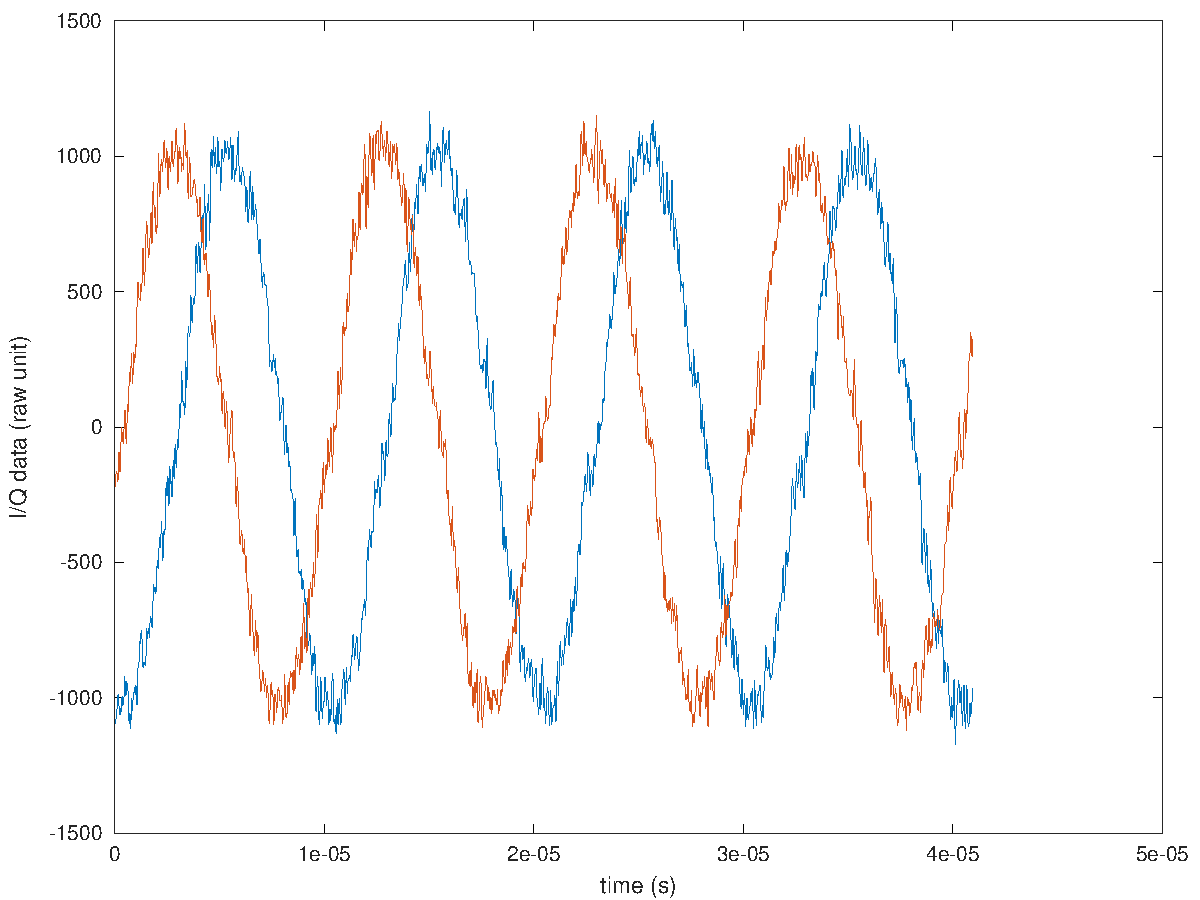
\includegraphics[width=\linewidth]{iio_iq_data.pdf}
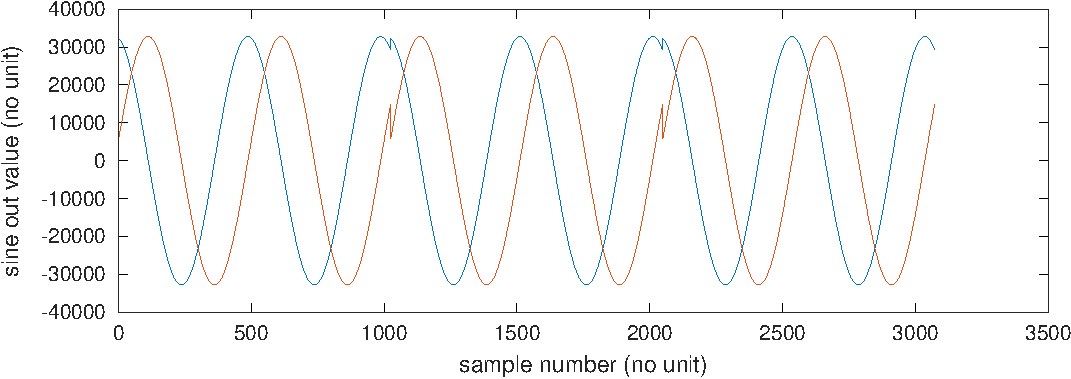
\includegraphics[width=\linewidth]{NCO.pdf}
%\end{minipage}\hfill
%\begin{minipage}[c]{0.49\linewidth}
%	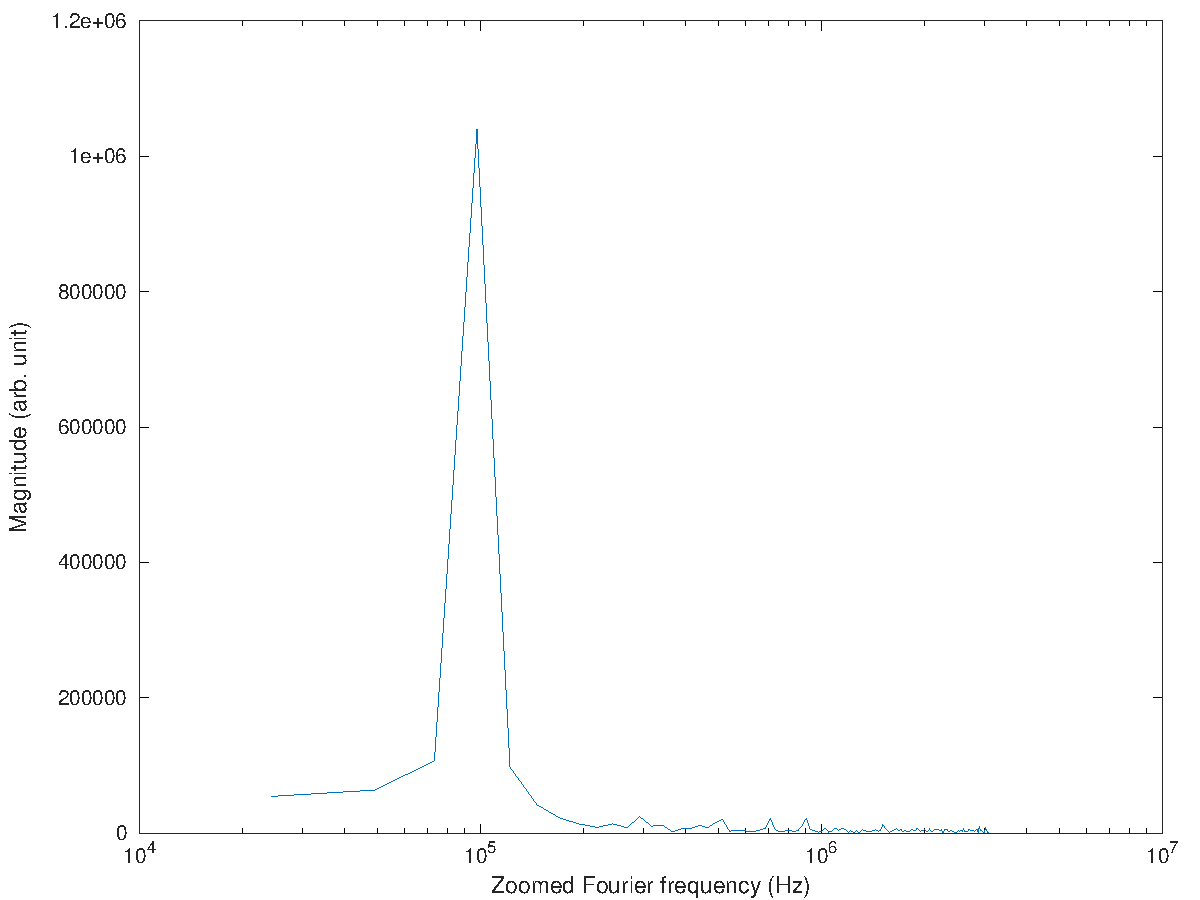
\includegraphics[width=\linewidth]{iio_fft_iq_data.pdf}
%\end{minipage}
\caption{Collected I/Q datasets. The 500~samples/period match the expected sampling
rate of 5~MS/s as a 100~kHz sine wave is generated by the NCO. Three successive (discontinuous)
datasets were collected.}% Right: Fourier transform.}
\label{nco}
\end{figure}

%-------------------------------------------------------
\section{PlutoSDR data stream $\to$ RAM $\to$ Userspace}
%-------------------------------------------------------
This second tutorial is a demonstration of the compatibility of the OSCIMP
ecosystem with the use of the existing Pluto HDL.
Once complete, you should be able to plug any DSP task to the initial design and
perform extra processing chains (Figs. \ref{chain1} and \ref{chain2}).

\begin{figure}[h!tb]
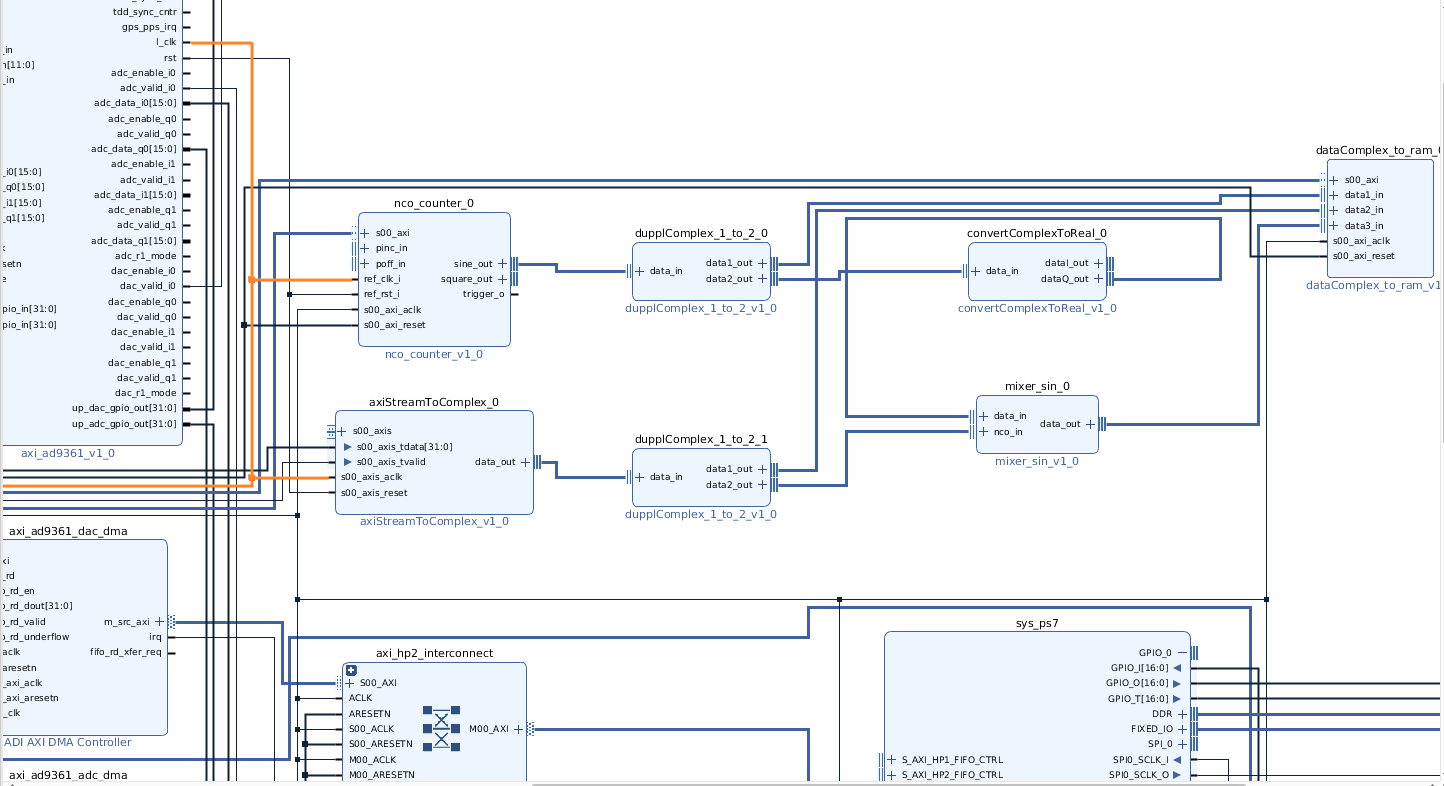
\includegraphics[width=\linewidth]{2.png}
\caption{Signal processing chain as defined in the Vivado 2018.3 graphical user
interface (added blocks are on the top right and include the nco\_counter, 
axiStreamToComplex, two duppComplex, convertComplextoReal, mixer\_sin and 
finally dataComplex\_to\_ram).}
\label{chain1}
\end{figure}

This time, since data from the AD9363 will be used in the flow chart, a consistent
clocking and signal reset distribution must be used:
\begin{itemize}
\item connect {\tt ref\_clk\_i} of the {\tt nco\_counter} to the {\tt axi\_ad9361} IP
{\tt l\_clk} (as is the {\tt s00\_axis\_aclk} of the {\tt axiStreamToComplex} block)
\item connect {\tt ref\_rst\_i} of the {\tt nco\_counter} to the {\tt axi\_ad9361} IP
{\tt rst} (as is the {\tt s00\_axis\_reset} of the {\tt axiStreamToComplex} block)
\item these clock and reset signals are then propagated to the other processing blocks through
their interfaces.
\end{itemize}

Failing to use these connections will result in timing errors including negative WNS and TNS
values related to the fact that the mixer is fed data from two different clock domains -- 100~MHz
for the AXI bus and 50~MHz for the AD9361.

\begin{figure}[h!tb]
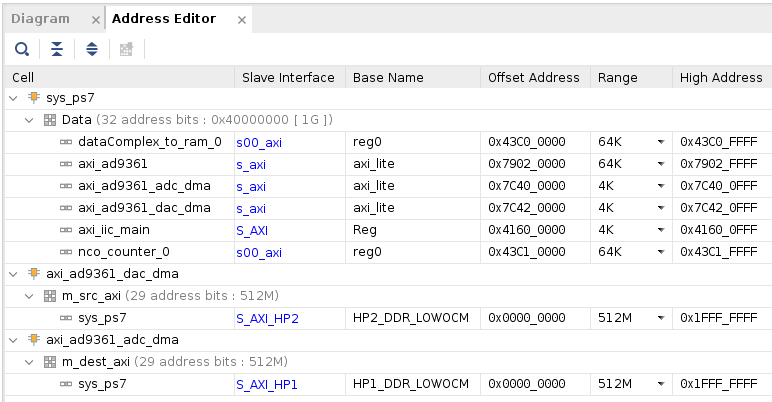
\includegraphics[width=\linewidth]{address.png}
\caption{Address map generated by Vivado: the devicetree source file must match
this configuration for the Linux drivers to reach registers at the right addresses.}
\label{chain2}
\end{figure}

Three datastreams lead to the DataToRAM block: the (complex) NCO output as addressed 
previously, the raw ADC (complex) data resulting from the I/Q demodulation within 
the AD9363 RF frontend, and the output of the mixer of the NCO with the ADC I/Q stream.
Since the ADI ADC is fed to a FIR decimator with no interface on the AXI Stream bus,
a direct connection to the axiStreamToComplex block is possible. Since the complex
valued output exhibits an interface, the resulting stream must be dupplicated 
(dupplCompl) when multiple processing -- here communication and mixing -- are to be
performed on the complex valued datastreams.

The resulting datasets are plotted on Fig. \ref{openclosed}, left with the
PlutoSDR disconnected from its input (noise measurement on the ADC) and right with
the RF output connected to the input through a 10~dB attenuator.

\begin{figure}[h!tb]
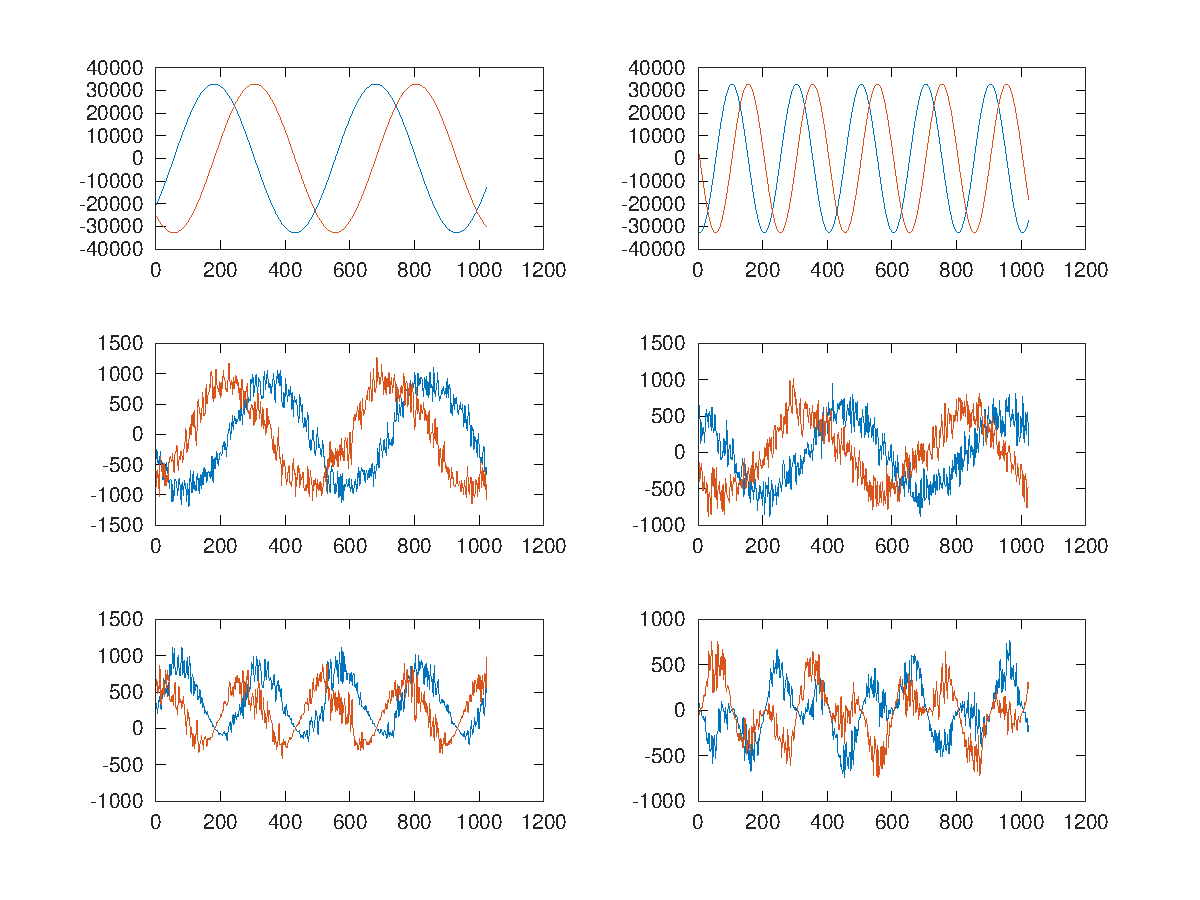
\includegraphics[width=\linewidth]{100kHz_250kHz}
\caption{Measurements results with a 100~kHz local oscillator (left) and with (right) a
250~kHz local oscillator, while in both cases the output is offset by 100~kHz from the
input. Top to bottom: NCO, measured I/Q streams, and mixer output.}
\label{openclosed}
\end{figure}

The original PlutoSDR used with GNU Radio remains functional despite the updated bitstream.
The same result than the one demonstrated from the OscimpDigital framework but running on the
host computer is shown in Fig. \ref{gnuradio}.

\begin{figure}[h!tb]
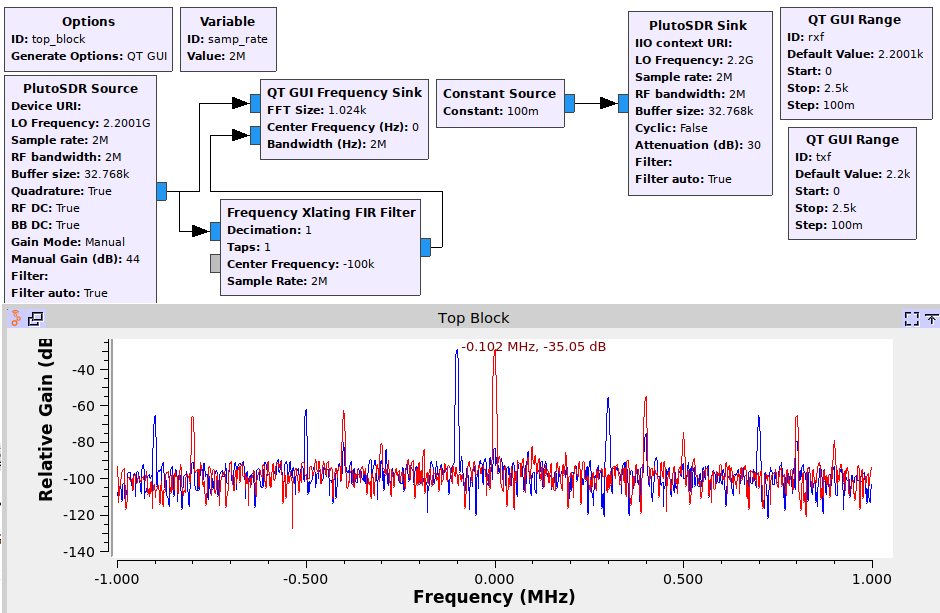
\includegraphics[width=\linewidth]{gnuradio.png}
\caption{GNU Radio flowchart accessing the PlutoSDR as source and sink with the updated
bitstream configuring the PL.}
\label{gnuradio}
\end{figure}

\section{TCL update of the original ADI PL configuration}

Rather than bothering with the graphical user interface, adding new functionalitites
brought by the OscimpDigital framework to the original ADI PL configuration file is most
efficiently achieved by updating the TCL script.

The TCL script provided by ADI is located at {\tt /somewhere/hdl/projects/pluto/system\_bd.tcl} and
must updated with the following:
\begin{itemize}
\item at the beginning of the file, insert the location of the OscimpDigital IP repository with
{\footnotesize
\begin{verbatim}
variable fpga_ip    $::env(OSCIMP_DIGITAL_IP)
set_property  ip_repo_paths [list ${fpga_ip} ${lib_dirs}] [current_project]
update_ip_catalog
\end{verbatim}
}
\item append the design with the additional blocks:
{\footnotesize
\begin{verbatim}
#nco
ad_ip_instance nco_counter nco
ad_ip_parameter nco CONFIG.DATA_SIZE 16
ad_ip_parameter nco CONFIG.COUNTER_SIZE 28
ad_ip_parameter nco CONFIG.LUT_SIZE 10

ad_connect axi_ad9361/rst nco/ref_rst_i
ad_connect sys_rstgen/peripheral_reset nco/s00_axi_reset
ad_connect axi_ad9361/l_clk nco/ref_clk_i

ad_cpu_interconnect 0x43C00000 nco

#dataComplex
ad_ip_instance dataComplex_to_ram data_to_ram
ad_ip_parameter data_to_ram CONFIG.NB_INPUT 1
ad_ip_parameter data_to_ram CONFIG.DATA_SIZE 16
ad_ip_parameter data_to_ram CONFIG.NB_SAMPLE 2048

ad_connect nco/sine_out data_to_ram/data1_in
ad_connect sys_rstgen/peripheral_reset data_to_ram/s00_axi_reset

ad_cpu_interconnect 0x43C10000 data_to_ram
\end{verbatim}
}
\item update the {\tt Makefile} by removing
{\footnotesize
\begin{verbatim}
M_DEPS += ../../library/xilinx/common/ad_iobuf.v
M_DEPS += ../../library/axi_ad9361/axi_ad9361_delay.tcl
\end{verbatim}
}
and replacing with
{\footnotesize
\begin{verbatim}
M_DEPS += $(ADI_HDL_DIR)/library/xilinx/common/ad_iobuf.v
M_DEPS += $(ADI_HDL_DIR)/library/axi_ad9361/axi_ad9361_delay.tcl
\end{verbatim}
}
with {\tt ADI\_HDL\_DIR} set to the {\tt /somewhere/hdl/} location,
\item 
in the {\tt Makefile}, remove
{\footnotesize
\begin{verbatim}
include ../scripts/project-xilinx.mk
\end{verbatim}
}
and replace with
{\footnotesize
\begin{verbatim}
include $(ADI_HDL_DIR)/projects/scripts/project-xilinx.mk
\end{verbatim}
}
\item in the {\tt system\_project.tcl}, replace
{\footnotesize
\begin{verbatim}
source ../scripts/adi_env.tcl
\end{verbatim}
}
with
{\footnotesize
\begin{verbatim}
variable adi_hdl_dir $::env(ADI_HDL_DIR)
source $adi_hdl_dir/projects/scripts/adi_env.tcl
\end{verbatim}
}
\end{itemize}

Following these updates, {\tt make} with synthesize the bitstream which can be
used as described earlier in the text to generate the {\tt .frm} and {\tt .dfu}
images to reflash the PlutoSDR.
\end{document}
